\chapter{Implementation}\label{sec:implementation}

This section details the implementation of the software which was developed for this project, which had the requirement of being able to accurately calculate the J-integral and stress intensity factor for a crack, using finite element analysis results generated via a commercial software package. The rationale for the methods and tools used is provided, followed by a brief summary of the architecture of the software. Finally, the implementation of the software itself is described, which is broadly split into the creation of the finite element model, the export of the analysis results from the commercial software package to a raw data format, and the calculation of the J-integral and stress intensity factor from these exported results.

\newpage
\section{Methods \& Tools}

\subsection{Method Selection}

As discussed in \S\ref{sec:mesh_meshfree}, the finite element method is the most commonly used method in industry for performing crack propagation calculations, and has the widest selection of commercial software, the broadest range of competent practitioners, and the most comprehensive set of validation data. Therefore, the finite element method was selected as the most suitable method for use in the implementation of this software, rather than a mesh-free method or an alternative mesh-based method. The standard element formulation was also selected -- rather than an enriched formulation such as XFEM -- as it has been demonstrated to be able to provide sufficiently accurate results for the stress intensity factor when using a tetrahedral mesh, while minimising additional complexity \cite{nejati_use_2015}. The equivalent domain integral method was selected as the most suitable method, due to its higher robustness compared to direct methods, and its ability to generate results from only a single finite element analysis run.

\subsection{Software Selection}

There are many different software packages available which are able to perform crack propagation calculations using finite element analysis. These can be broadly split into  widespread, general-purpose packages, smaller and more niche packages, and in-house packages developed within engineering companies for specific purposes.

The general-purpose packages are developed by large companies, and are not sector-specific -- these include NASTRAN, HyperWorks, Ansys, and Abaqus. These packages usually deal with the end-to-end process, where geometry definition, meshing, analysis, and post-processing can all be performed using the same piece of software. Modules are generally available for specialised types of analysis -- such as crack propagation analysis. However, these modules are less comprehensive than those available in more niche packages, due to the one-size-fits-all approach taken. Due to the popularity of these packages and the resources available to the developers, tools are often provided which can be used by customers to extend the software further by developing custom scripts.

Other -- more niche -- packages are also available, which are generally tailored towards a small set of specific applications such as crack propagation. These packages utilise a more established software package for their base feature set -- for example, meshing the geometry and solving the differential equations -- while incorporating new features such as the ability to re-mesh automatically, or the ability to incorporate additional post-processing and visualisation of the results. Some of the available software in this category for crack propagation specifically include Zentech, BEASY, and Z-Cracks. These packages can be very useful as they provide additional features which are not available in the more common packages, and can be used off-the-shelf by customers. However, they generally aren't as extensible as the larger software packages.

For some specific applications, even niche software packages may not be able to meet the needs of a customer, and this can necessitate the development of bespoke analysis tools within an engineering company itself. These tools can be costly to develop and maintain, but can be necessary for certain applications specific to a particular company. As these tools are developed internally and contain a company's valuable intellectual property, they are generally not available to the public for use. They provide maximum flexibility, as the company is free to develop them to meet whichever needs they may require. These may be standalone tools, or extensions for commercial software packages.

The software selected for the development of the script was Abaqus (v2023). Abaqus is a finite element analysis software package that is ubiquitous within industry -- particularly for non-linear structural analysis. Abaqus provides the Abaqus Scripting Interface -- this is an application programming interface (API) which can be used to interact with Abaqus programatically, and perform tasks such as generating models, exporting results, and performing post-processing. Calculations can either be performed within Abaqus, or the analysis results data can be exported in order to perform the calculations outside of Abaqus.

\subsection{Language Selection}

The Abaqus API supports two programming languages -- Python and C++. Python is a high-level interpreted language, which offers a relatively simple development process along with a large collection of libraries for data processing and scientific computing. The key advantage of Python is that it can shorten the development time required to produce a viable piece of software -- however, as a high-level interpreted language, its performance when dealing with large-scale computations is relatively lacklustre. This can somewhat be compensated for when using high-performance libraries such as NumPy and SciPy which are written in more performant languages such as C, C++, and FORTRAN \cite{numpy_performance_nodate}.

C++, on the other hand, is a compiled language that operates at a lower level than Python, and which is commonly used in the development of computationally demanding software due to its high performance and ability to manually manage memory allocation. However, software developed using C++ generally requires a longer development time when compared to Python because of its increased complexity and the absence of high-level features available in Python. An alternative approach considered was to use either Python or C++ to create the validation model and export the results from Abaqus, while using a separate language to perform the analysis. This approach would have potentially been the most flexible -- however, using multiple languages would have increased the overall complexity of the program \cite{zehra_comparative_2020}.

The decision was made to use Python for the entirety of the development process, including the model generation, the results export, and the analysis. This allowed simplicity to be maximised while minimising the development time and complexity. As the test cases were fairly simple, the benefits of developing in C++ would not have been fully realised, while the use of high-performance Python libraries to perform the analysis allowed the lower performance of Python to be somewhat mitigated. Using two languages for the development was rejected as being too complex for a proof-of-concept project. If the software were eventually to be extended and used within a production environment, it would be relatively straightforward to translate the code into a higher-performance language, given that the program's logic had already been implemented and tested.

\newpage
\section{Architecture}

The software was developed using an object-oriented approach whereby methods were separated into different classes -- each with a separate and well-defined purpose. For the sake of simplicity, a combination of command-line arguments and a \texttt{config.ini} configuration file were used to specify the options for each run. The software was broadly split into three modular sections in order to maximise flexibility -- the creation of the validation model, the export of the results, and the performance of the calculations. This approach meant, for example, that it was possible to run multiple analyses on the same set of Abaqus results -- using a different set of parameters -- without having to re-create and re-run the model each time. A fourth section of the code managed the running of the software itself. The four sections of the software were managed by four separate classes:

\begin{itemize}
	\item \texttt{create\_model.py} -- Generates a validation model and runs an analysis job within Abaqus, using parameters defined within the \texttt{config.ini} configuration file. This step was managed by the \texttt{model.py} class.
	\item \texttt{export\_results.py} -- Exports the results from the proprietary Abaqus Output Database (ODB) file format to an open JSON format, so that the analysis could be run in a stand-alone manner, without needing Abaqus to be open.
	\item \texttt{analyse\_results.py} -- Performs all the calculations necessary to determine the J-integral and stress intensity factor of the crack using the exported results, and saves the calculation results to CSV and JSON files.
	\item \texttt{runner.py} -- Performs administrative duties such as parsing the command line arguments, creating directories for each individual run, and calling the classes for each part of the analysis using the correct arguments.
\end{itemize}

The overall architecture of the software is presented in Figure \ref{fig:software_architecture}. Further information on how to actually run the software is provided within the \texttt{readme.md} file, available in the GitHub repository for the project, and in the appendix of this document. A link to the GitHub repository is also provided in the appendix (\S\ref{sec:appendix}).

\begin{figure}[H]
	\centering
	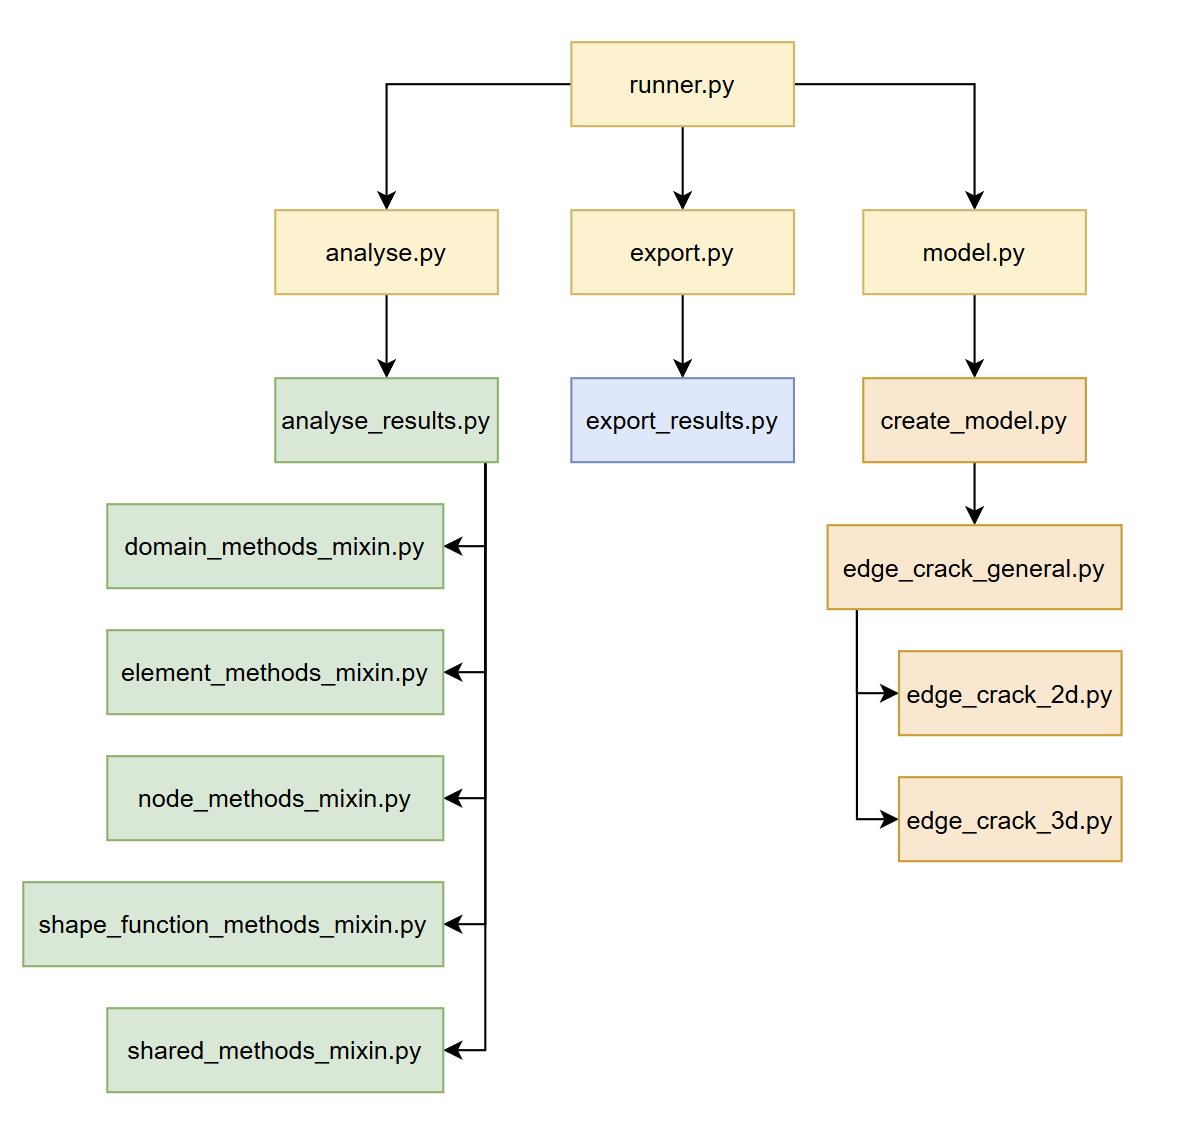
\includegraphics[width=\textwidth]{software_architecture.png}
	\caption{Architecture diagram of the J-integral calculation software developed for this project, demonstrating the separation of functionality into four sections. The files relating to the run manager, model creation, results export, and results analysis are in yellow, orange, blue, and green respectively.}
	\label{fig:software_architecture}
\end{figure}

\newpage
\section{Model Creation}\label{sec:fea_modelling}

As discussed in \S\ref{sec:case_study}, a through-thickness edge crack in a finite plate was selected as the case study to demonstrate the validity of the software. This is because it was relatively simple to model, and was represented well in the literature -- with both analytical and numerical solutions readily available for comparison. In order to provide maximum traceability and reproducibility of the results, Python scripts were developed which could generate the model parametrically, based on a configuration file. This allowed factors such as the applied stress, plate dimensions, crack length, and mesh density to be adjusted quickly in order to investigate the impact of these factors on the results of the analysis.

\subsection{Units \& Geometry}

The set of units used for the model were $N$, $mm$, and $MPa$. This meant meant that the units for the J-integral were in $N\ mm^{-1}$, and the units for the stress intensity factor were in $MPa\ \sqrt{mm}$. A plate with an aspect ratio of $1:2$ (width to height) was selected, as this geometry was found to be well-represented in the literature. A unit thickness of 1.0 mm was used -- for both the 2D and 3D models -- in order to ensure plane stress conditions. The geometry of the plate is presented in Table \ref{tab:part_geometry}, for the reference configuration. The crack length was varied between 2 mm and 25 mm as part of the analysis, in order to understand the impact of crack length on the J-integral and stress intensity factor. However, an initial crack length of 10 mm was used as the reference configuration, in order to validate the modelling approach.

\renewcommand{\arraystretch}{1.5}

\begin{table}[htbp]
	\centering
	\caption{Reference geometry for the 2D and 3D edge-cracked models.}
	\label{tab:part_geometry}
	\begin{tabular}{|c|c|c|c|}
		\hline
		\textbf{Height (mm)} & \textbf{Width (mm)} & \textbf{Thickness (mm)} & \textbf{Crack Length (mm)} \\ \hline
		100.0 & 50.0 & 1.0 & 10.0 \\ \hline
	\end{tabular}
\end{table}

\subsection{Coordinate System}

A common approach when performing crack-related finite element analysis is to define a separate coordinate system for the crack, so that measurements such as nodal coordinates and displacements can be described in terms relative to the crack tip. However, because this work used a model which was parametrically generated through via the Abaqus API, the global coordinate system was used instead for increased simplicity. The crack tip was placed at the origin of the global coordinate system, and the rest of the part geometry was created relative to the crack tip. A configuration parameter -- \texttt{crack\_tip\_coordinates} -- was also specified, which allowed for the use of different coordinate system origins to be more easily integrated into future updates.

\newpage
\subsection{Material}

The material used for the model was not a significant parameter when calculating the stress intensity factor, as the stress intensity factor is a material-independent property which only considers the crack length, part geometry, and applied stress. Only the critical stress intensity factor -- which quantifies the fracture toughness of a material -- is material-specific, and this parameter was not necessary for the purposes of this work. Therefore, aluminium was arbitrarily selected as the material to be used, and was specified in Abaqus using a linear-elastic material type, along with the parameters presented in Table \ref{tab:material_params}.

\begin{table}[htbp]
	\centering
	\caption{Parameters used to specify the linear-elastic material in Abaqus.}
	\label{tab:material_params}
	\begin{tabular}{|c|c|c|}
		\hline
		\textbf{Material Name} & \textbf{Young's Modulus - E (MPa)} & \textbf{Poisson's Ratio - \bm{$\nu$}} \\ \hline
		Aluminium & 72,000 & 0.3 \\ \hline
	\end{tabular}
\end{table}

\subsection{Partitioning}

The model was partitioned in order to be able to increase the element size near the crack tip to maximise accuracy, while maintaining a coarse element size away from the crack tip to minimise computation time. Three horizontal partitions were first created, both above and below a central partition which contained the crack. The first partition was placed at a distance equal to the crack length, and the other partitions were placed based on a bias ratio defined in the configuration, which was used to alter their relative sizes. The central section was then partly partitioned in order to introduce the crack. A line equal to double the crack length was defined from the left edge at the middle of the central partition. This was then further partitioned into two lines of equal length via the introduction of a point at the halfway mark. Finally, a crack seam was assigned to the partition line representing the crack, to enable the nodes in that area to be separated during the analysis and allow the crack to open. Figure \ref{fig:2d_fea_model_meshed_unmeshed} shows the partitioning strategy used for the baseline 2D analysis, with a crack length of 10 mm and a horizontal partition bias of 1.5. The first yellow plane passes through the crack tip, while the second yellow plane passes through the end of the linear partition used to refine the mesh ahead of the crack tip.

\begin{figure}[H]
	\centering
	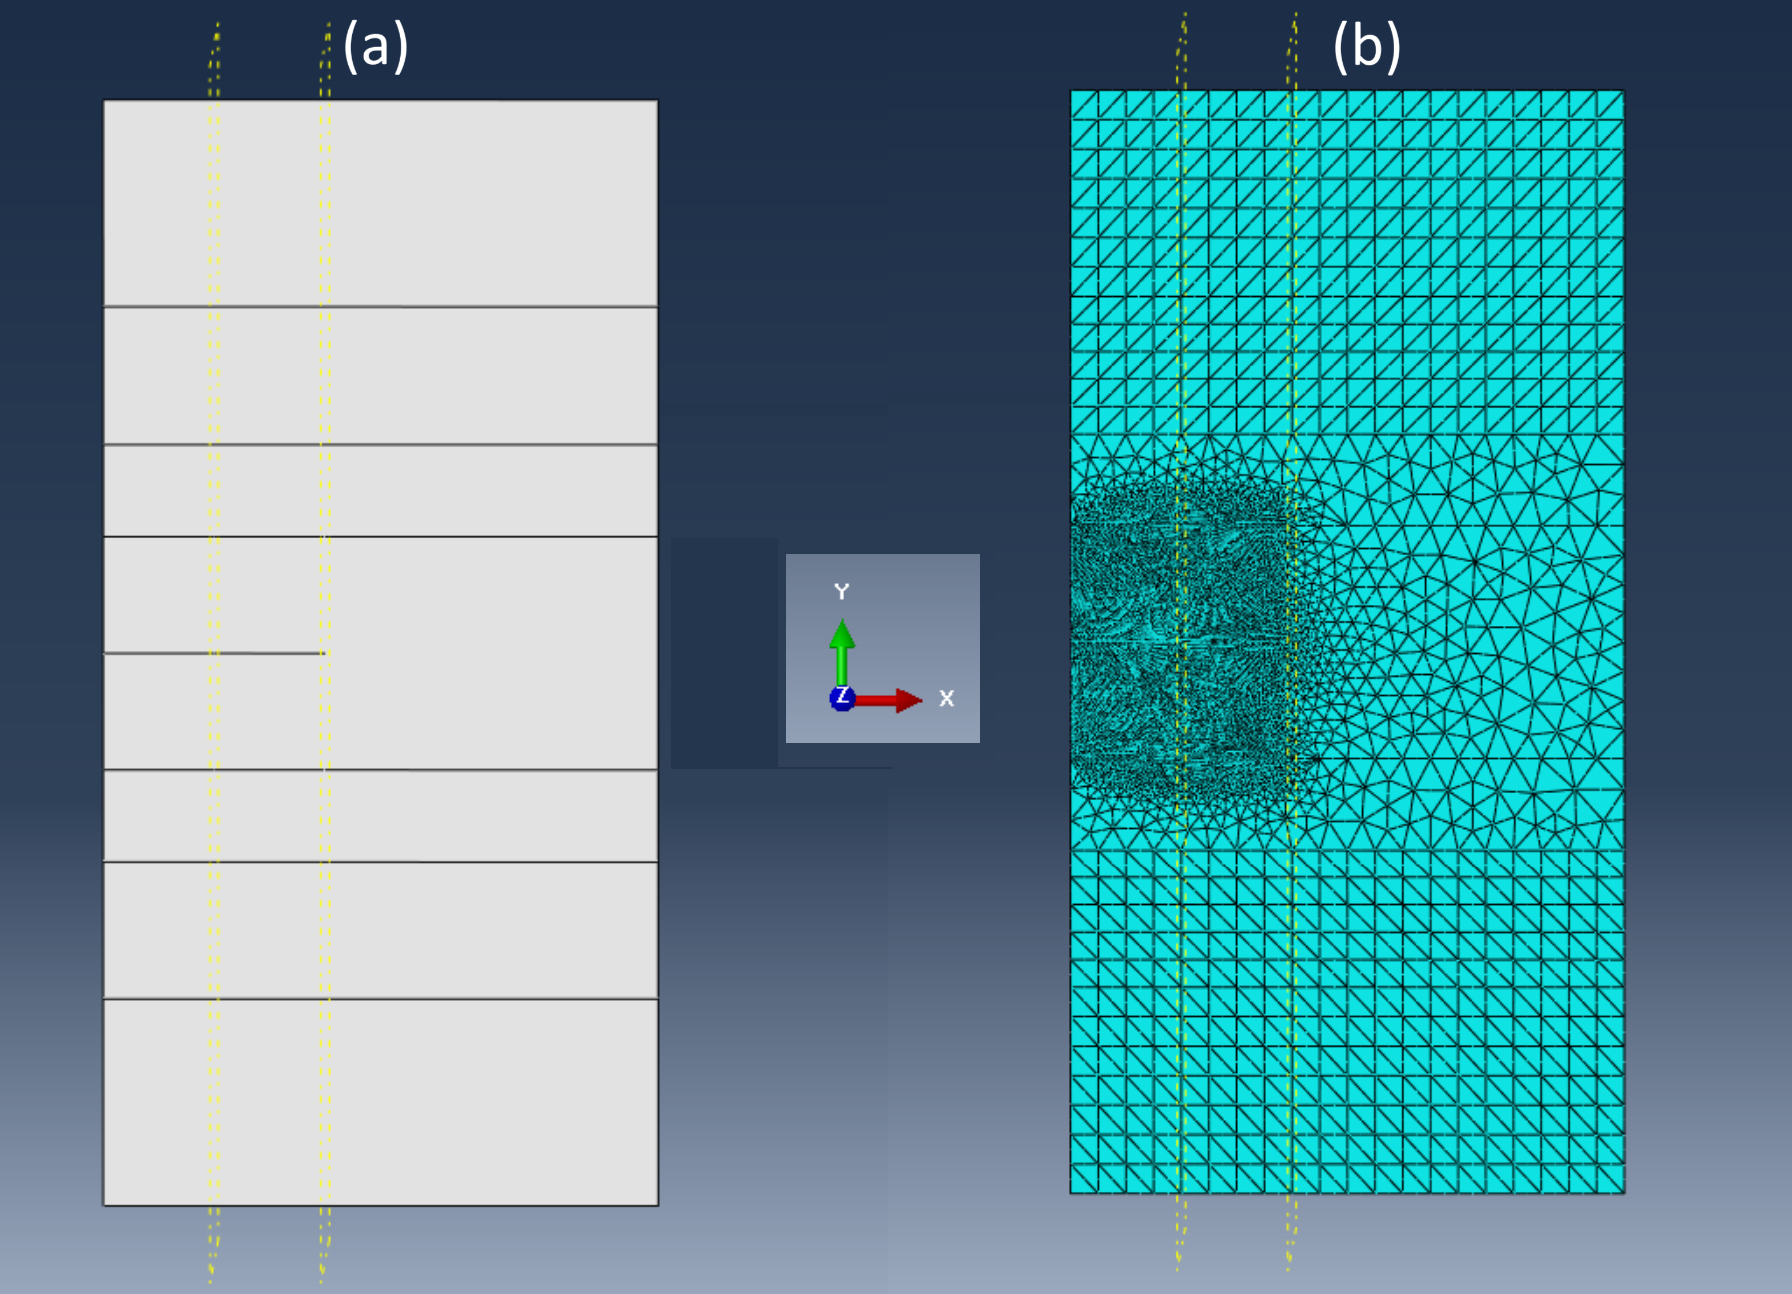
\includegraphics[width=13cm]{2d_model_meshed_unmeshed.png}
	\caption{Screenshot of the 2D edge crack model within Abaqus. The first image (a) shows the partitioned geometry, while the second image (b) shows the meshed model.}
	\label{fig:2d_fea_model_meshed_unmeshed}
\end{figure}

\subsection{Meshing}

Initially, a radial mesh and partitioning scheme was used for the 2D model to maximise the structure of the mesh and the accuracy of the results. However, it was found that this meshing strategy did not transfer over to the 3D model, as the numerous partitions meant that the auto-mesher struggled to generate the triangular boundary elements necessary to join the separate meshes of each partition. Therefore, the meshing strategy was altered to one which was able to mesh both the 2D and 3D models automatically, while still enabling mesh refinement near the crack tip. Figure \ref{fig:2d_fea_model_meshed_strategy} shows the mesh seeds for the reference model. The parameter \texttt{crack\_element\_count} was used to define the number of elements along the biased edges, and was set at 50. The parameter \texttt{crack\_element\_bias} was used to set the bias ratio along the biased edges, and was set at 2. Finally, the \texttt{through\_thickness\_element\_count} parameter was used to define the number of through-thickness elements within the crack tip partition -- for the 3D model only -- and was set at 5. This meant that the mesh density increased towards the crack tip, while remaining coarse in the areas remote from the crack tip. This allowed the high stress gradients near the crack tip to be captured as accurately as possible, while minimising the solution time of the model.

\begin{figure}[H]
	\centering
	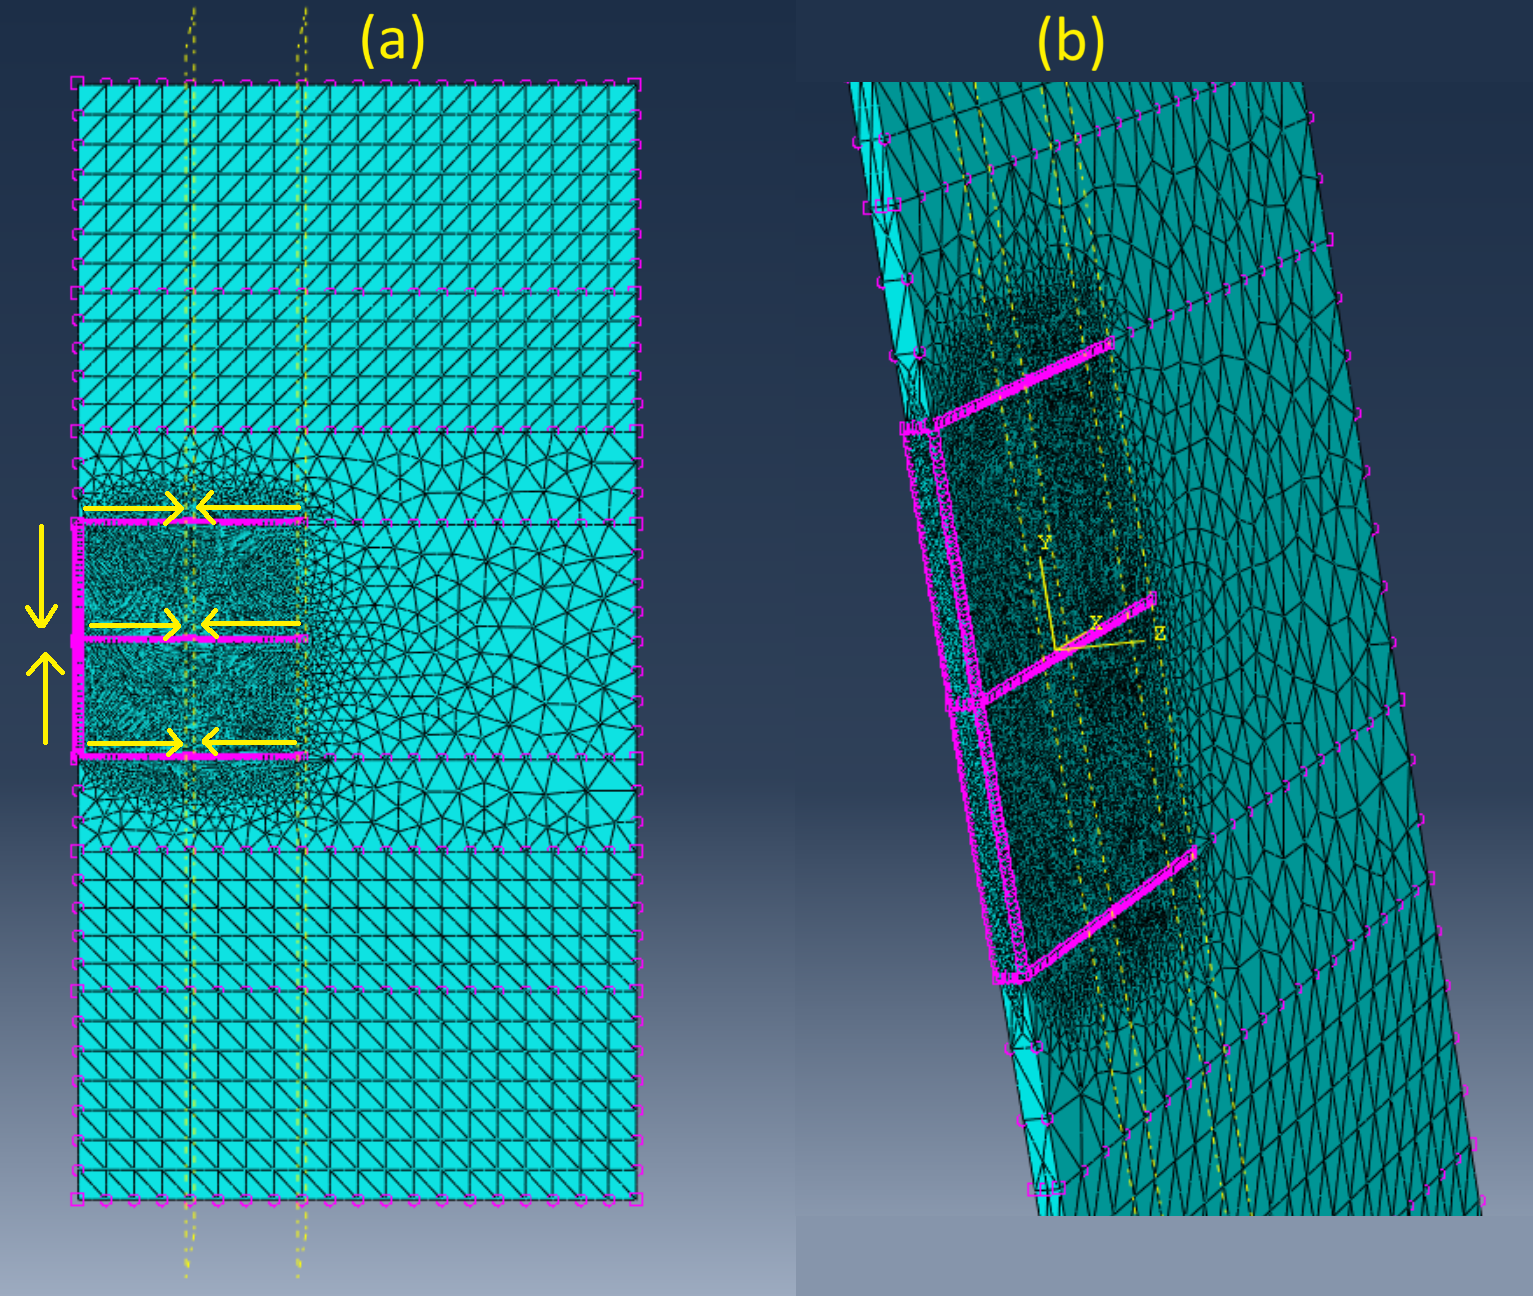
\includegraphics[width=13cm]{2d_model_meshed_strategy.png}
	\caption{Screenshot of the 2D and 3D models within Abaqus, showing the element biasing. The yellow arrows show the biased edges, along with the direction of bias, while the unlabelled edges show the coarse mesh seeds. The first image (a) shows the biasing of the 2D model, while the second image (b) shows the biasing of the 3D model.}
	\label{fig:2d_fea_model_meshed_strategy}
\end{figure}

For the 2D model, CPS6 elements were specified, which are six-node quadratic triangular shell elements. For the 3D model, C3D10 elements were specified, which are ten-node quadratic tetrahedral elements. Quadratic elements have been demonstrated to improve accuracy when compared to linear elements -- particularly in areas of high stress gradients, such as the tip of a crack \cite{kuna_finite_2013}.

\subsection{Loading \& Boundary Conditions}

For the 2D model, sets were created for the top edge, the bottom edge, and the bottom-left vertex, while for the 3D model, sets were created for the top face, the bottom face, and the bottom-left edge. A fixed support was applied to the bottom-left set to constrain rigid-body motion without over-constraining the model, and a roller support was applied to the bottom set to constrain displacements in the y-direction. A uniform negative pressure load of 100 MPa was then applied to the top edge or surface, to represent the applied uniform stress, and model a pure mode 1 crack opening scenario.

\begin{figure}[H]
	\centering
	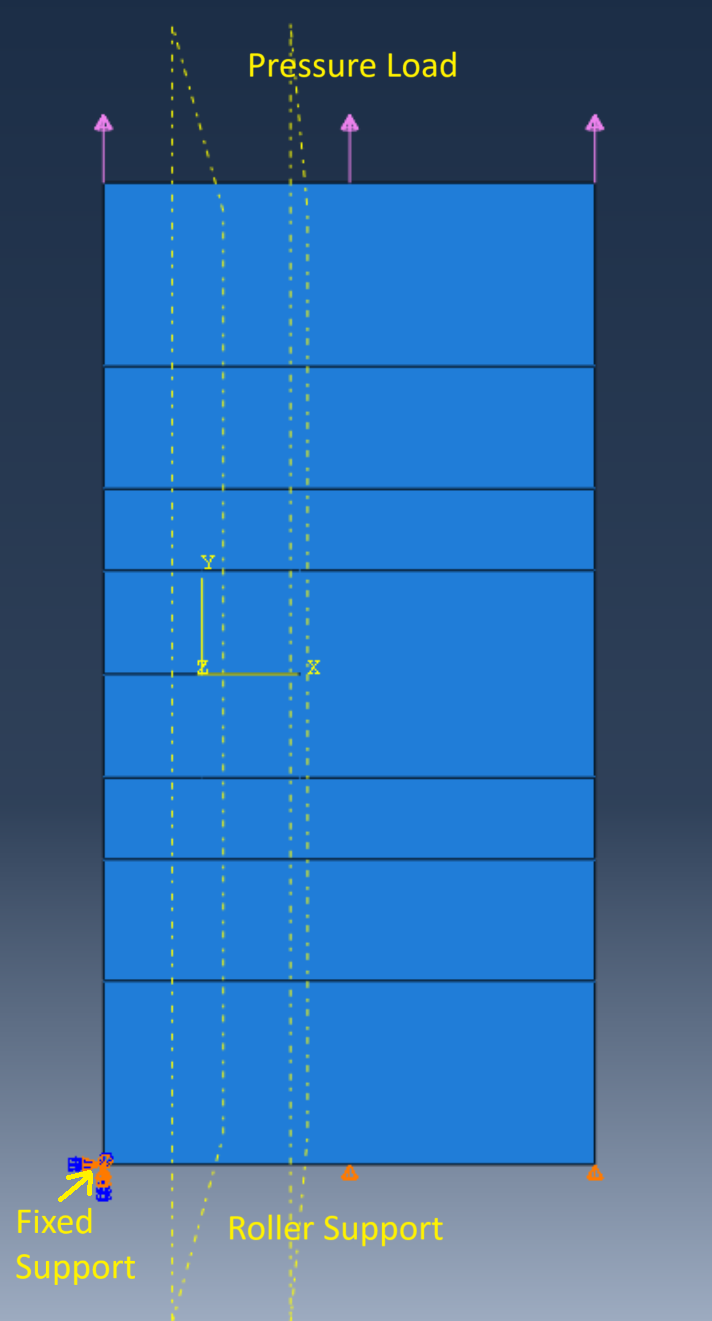
\includegraphics[width=8cm]{2d_model_loading_bcs.png}
	\caption{Screenshot of the 2D edge crack model within Abaqus, showing the loading and boundary conditions. A fixed support was applied to the bottom-left corner, a roller support was applied to the bottom edge, and a pressure load was applied to the top edge.}
	\label{fig:2d_fea_model_loading_bcs}
\end{figure}


\newpage
\section{Results Export}

Abaqus outputs results in the output database (ODB) format. This is a proprietary file format which requires an Abaqus license to open. Although the J-integral calculations could have been performed by directly accessing the ODB file using the Abaqus API, it was decided instead to use the Abaqus API to export the required results from the ODB to a JSON file, which could then be used to perform the calculations outside of Abaqus. This approach was selected as it maximised the flexibility of the tool -- allowing the calculations to be performed without an Abaqus license, provided that a set of exported results were already available to the user. The development time for the software was reduced by simplifying the debugging process, and allowing the use of Python 3 libraries rather than being limited solely to the Python 2 libraries available within the version of Abaqus used for the analysis. The results export was split into \texttt{node\_data}, and \texttt{element\_data}, which were used as the top-level keys within the JSON output file. The structure of the JSON file is given below.

\begin{verbatim}
{
    "node_data": {
        "node_label":
            "coordinates_original": [],
            "displacement": [],
            "connected_elements": []
    },
    "element_data": {
        "element_label":
            "stress_tensor": {"integration_point": []}
            "strain_tensor": {"integration_point": []},
            "connected_nodes": []
    }
}
\end{verbatim}

\newpage

A more detailed description of the data stored within each key is also provided here.

\begin{itemize}
	\item Node Data:
	\begin{itemize}
		\item \texttt{"node\_label"} - The numerical identifier assigned to the node by Abaqus.
		\item \texttt{"coordinates\_original"} - A 2x1 (in 2D) or 3x1 matrix (in 3D), containing the original (undeformed) coordinates of the node in the global coordinate system.
		\item \texttt{"displacement"} - The 2x1 (in 2D) or 3x1 (in 3D )matrix, containing the displacement vector for the node.
		\item \texttt{"connected\_elements} - A list of the labels of all elements connected to the node.
	\end{itemize}
	\item Element Data:
	\begin{itemize}
		\item \texttt{"element\_label"} - The numerical identifier assigned to the node by Abaqus.
		\item \texttt{"stress\_tensor"} - A 2x2 (in 2D) or 3x3 (in 3D) matrix for each integration point within the element, containing the stress tensor at that integration point, in tensorial form.
		\item \texttt{"strain\_tensor"} - A 2x2 (in 2D) or 3x3 (in 3D) matrix for each integration point within the element, containing the strain tensor at that integration point, in tensorial form.
		\item \texttt{"connected\_nodes"} - A list of the labels of all nodes connected to the element.
	\end{itemize}
\end{itemize}

According to the Abaqus theory manual \cite{systemes_122_nodate}, stresses are output in their tensorial form as true (Cauchy) stresses, while strains are output in their engineering form, using engineering shear strains. It was therefore necessary to convert the engineering strain into the tensorial strain by halving the shear strain components. This was performed during the export rather than at a later stage for the sake of simplicity.

\newpage
\section{Results Analysis}

\subsection{Analysis Summary}

The calculation of the J-integral and stress intensity factor was performed using the JSON file which was generated from the Abaqus ODB file during the export stage. A summary of the analysis process is provided below, while the steps are described in more detail in the following sections.

\begin{itemize}
	\item Filter the data to retain only the elements and nodes that lie within the maximum integral domain.
	\item Calculate the displaced nodal coordinates for each node.
	\item Define the integration domains as annular regions around the crack tip.
	\item Compute the shape functions and shape function derivatives for the element type in the natural coordinate system.
	\item For each integration point of each element, calculate:
	\begin{itemize}
		\item The coordinates in the global coordinate system.
		\item The Jacobian matrix and determinant.
		\item The strain energy density.
		\item The displacement gradients.
		\item For each domain, calculate:
		\begin{itemize}
			\item The value and derivative of the weight function ($q$ and $\frac{dq}{dr}$).
			\item The contribution of that integration point to the total J-integral for the domain.
		\end{itemize}
	\end{itemize}
	\item Then, for each domain:
	\begin{itemize}
		\item Sum the J-integral contribution from each element for each domain, to calculate the total J-integral.
		\item Use the J-integral to calculate the stress intensity factor.
	\end{itemize}
	\item Calculate the stress intensity factor analytically, using the analytical formula for the configuration parameter $\beta$ for an edge-crack in a finite plate.
	\item Calculate an analytical value for the J-integral, using the analytically calculated stress intensity factor.
	
\end{itemize}

\newpage
\subsection{Data Filtering}

The JSON file generated from the Abaqus ODB file contained data on all of the elements and nodes within the analysis, to provide maximum traceability of the results. However, only the data for elements and nodes close to or within the radius of the largest integral domain was required to perform the analysis. Therefore, the first step was to filter the data to include only the relevant elements and nodes. This improved the performance of the software by minimising the amount of data that was read into memory, and ensured that resources were not wasted on calculating parameters for irrelevant elements and nodes. The configuration parameter \texttt{domain\_r\_max\_factor} was used to define the radius of the largest integral domain, as a fraction of the crack length. An additional factor was then applied to this to ensure that the data around the outside of the largest domain was also captured -- to avoid, for example, capturing data for an element near the outside of the domain but failing to capture the data on all its connected nodes.

\subsection{Displaced Nodal Coordinates}

The nodal data obtained from Abaqus included the original coordinates for each node, along with their displacement vectors. The displaced coordinates of each node were required for further calculation steps -- therefore, they were calculated using Equation \ref{eq:disp_nodal_coords}.

\begin{equation}\label{eq:disp_nodal_coords}
	\bm{x'} = \bm{x} + \bm{u}
\end{equation}

\begin{itemize}
	\item $\bm{x'}$ is a vector of size ($n_{dim}, 1$) containing the displaced nodal coordinates.
	\item $\bm{x}$ is a vector of size ($n_{dim}, 1$) containing the original nodal coordinates.
	\item $\bm{u}$ is a vector of size ($n_{dim}, 1$) containing the nodal displacements.
	\item $n_{dim}$ is the number of dimensions for the model.
\end{itemize}

\subsection{Integral Domain Definition}\label{sec:implementation_domains}

Two approaches for defining the integration domains were evaluated. Both approaches used multiple domains of gradually increasing size, using the parameters \texttt{domain\_r\_min}, \texttt{domain\_r\_max}, and \texttt{number\_of\_domains} to define the minimum and maximum radii of the domain, along with the total number of domains to use. The first domain for both approaches was a circle or cylinder (for the 2D and 3D models respectively) of radius $r_{min}$, which included all of the elements around the crack tip. Further domains were then generated -- with gradually increasing radii -- until $n_{domains}$ domains had been generated, with a final domain radius of $r_{max}$. The reason for using multiple domains for each analysis was to verify the domain-independence of the results. If the equivalent domain integral method had been implemented correctly, then minimal differences between the J-integral values obtained from each domain should have been observed. This was a key step in validating the outputs of the software.

The first domain approach utilised circles of increasing radius -- i.e. domain 2 included all of the integration points present in domain 1, along with additional integration points. This approach was found to be less accurate, as the elements very near to the crack tip were very highly represented -- becoming increasingly so as the domain size increased due to the use of the weight function. As standard (rather than quarter-point) elements were used at the crack tip, this approach was found to be very dependent on the mesh density near the crack tip.

The second approach utilised annular rings of increasing radius -- rather than circles -- meaning that each integration point only appeared in a single domain, with the crack tip elements only being represented within the first domain. This approach reduced the dependence of the results on the crack tip elements, since they only appeared in the innermost domain. This allowed the J-integral to be calculated using the more accurate stresses further away from the crack tip, and therefore improved the accuracy of the results. A comparison of the two approaches is presented in Figure \ref{fig:domain_approaches}.

\begin{figure}[H]
	\centering
	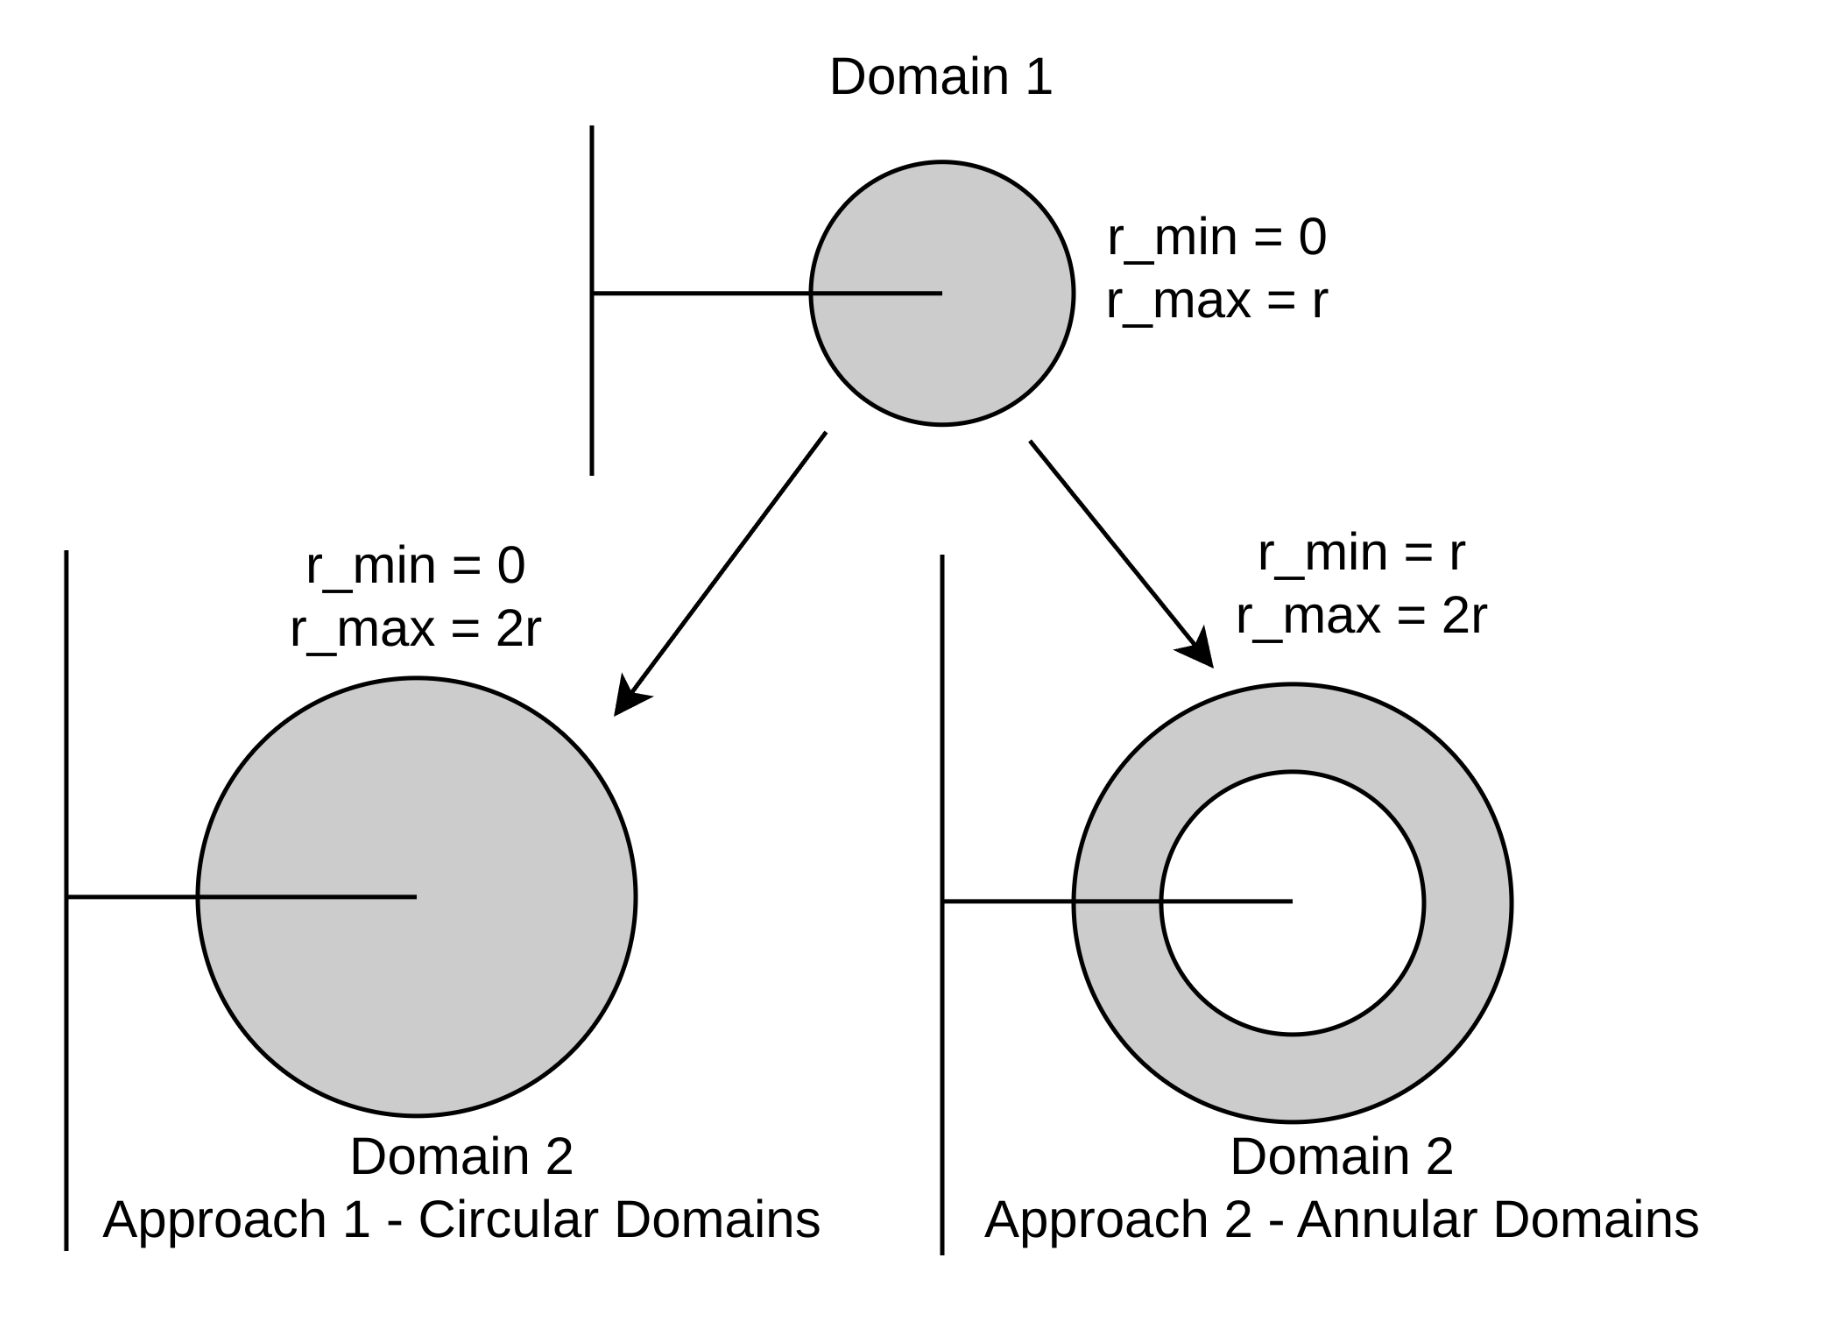
\includegraphics[width=11cm]{domain_approaches.png}
	\caption{Diagram showing the two tested domain definition approaches. Domain 1 is the same for both approaches. Domain 2 for Approach 1 expands the domain into a larger circle, while Domain 2 for Approach 2 instead uses an annular ring around domain 1.}
	\label{fig:domain_approaches}
\end{figure}

Elements were assigned to specific domains based on their nodal coordinates. Effectively, if a node lay within the domain boundaries, then all elements attached to that node were assigned to that domain. This meant that elements could appear in more than one domain -- for example, if two nodes of that element each lay in separate domains. However, the use of the weight function (discussed in \S\ref{sec:weight_functions}) ensured that each integration point was only represented in the J-integral calculation for a single domain. An integration point that was assigned to a domain but that did not actually lie within the boundaries of that domain would be assigned a weight of zero, and would therefore not affect the calculation. This method produced accurate results by allowing the use of stresses directly from the integration points, while avoiding any need to interpolate the stresses to other points within the element. The basic logic used to assign elements to each domain is described in the pseudo-code below.

\begin{verbatim}
	Define each annular domain based on a minimum and a maximum radius
	
	    For each element:
	        For each node attached to that element:
	            Get the distance between the node and and the crack tip
	            For each domain:
	                If the node lies within the domain:
	                    Add the element to the domain
	                    
	Filter each domain to ensure each element only appears once per domain	
\end{verbatim}

Figure \ref{fig:domain_elements} presents a visualisation of the assignment of integration points to a domain. Elements 1, 2, and 3 are all included in the domain since at least one node of each element lies within the domain boundary. However, the weight function means that the integration points that fall outside of the domain boundary (in red) do not contribute to the J-integral calculation, while the integration points within the domain (in green) do contribute.

\begin{figure}[H]
	\centering
	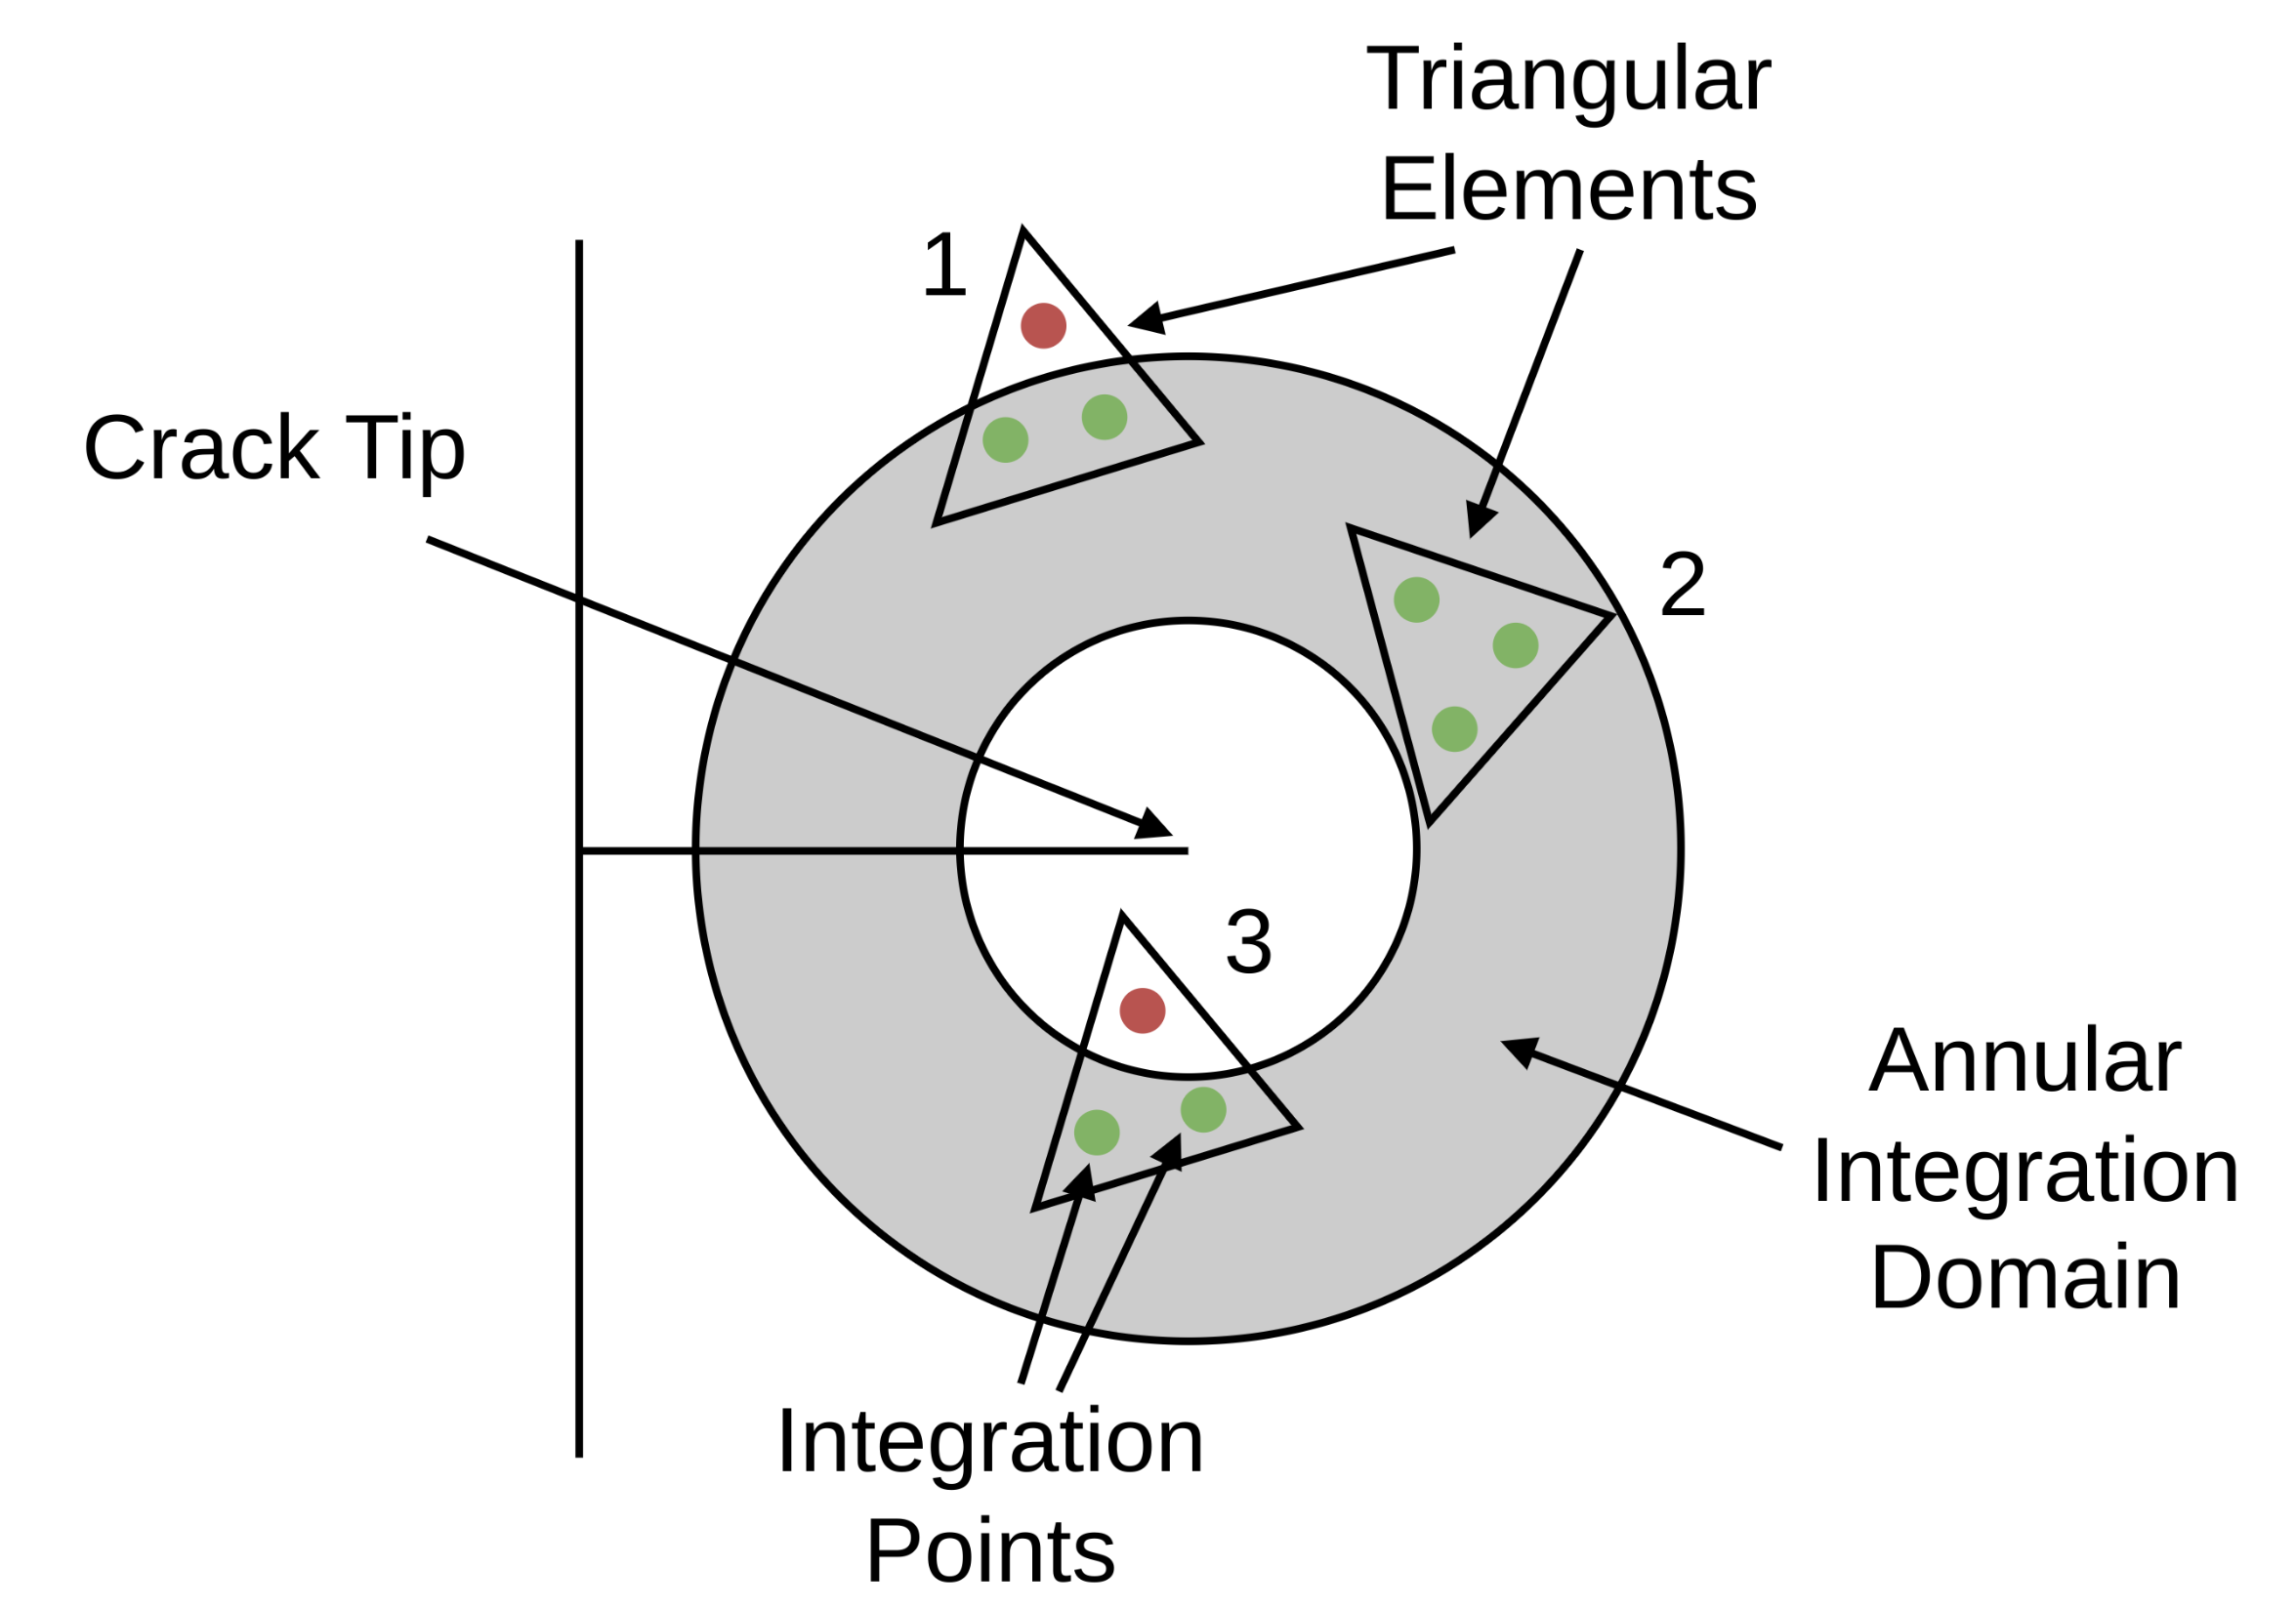
\includegraphics[width=12cm]{domain_elements.png}
	\caption{Diagram showing the filtering of integration points within a domain. All of the integration points of element 2 are included in the domain, while elements 1 and 3 have one integration point that falls outside the outer and inner boundaries of the domain respectively.}
	\label{fig:domain_elements}
\end{figure}

\newpage
\subsection{Shape Functions \& Derivatives}

Element shape functions are necessary in order to interpolate the field variables -- for example displacements, stresses, and strains -- at any point inside the element using the nodal data. For this project, they were used to determine the coordinates of the element integration points, which allowed the calculation of their weights. The derivatives of the shape function derivatives were also necessary to calculate the Jacobian matrices and determinants at each integration point and the displacement gradients. The element shape function expressions were obtained from the Abaqus Theory Manual \cite{systemes_326_nodate}, while the integration point coordinates in the natural coordinate system were obtained from the Code\_Aster documentation \cite{aster_111_nodate}.

The SymPy library was used to create symbolic representations of the shape functions in the natural coordinate system. These were then differentiated in order to obtain the shape function derivatives -- also in the natural coordinate system. Finally, the expressions were evaluated using the natural points for each integration point in order to obtain the coordinates of each integration point in the natural coordinate system. These values were saved within an array that could be used along with the specific nodal coordinate data for each element in future calculation steps. Figure \ref{fig:isoparametric_elements} shows the nodal numbering for the CPS6 and C3D10 elements utilised within this project.

\begin{figure}[H]
	\centering
	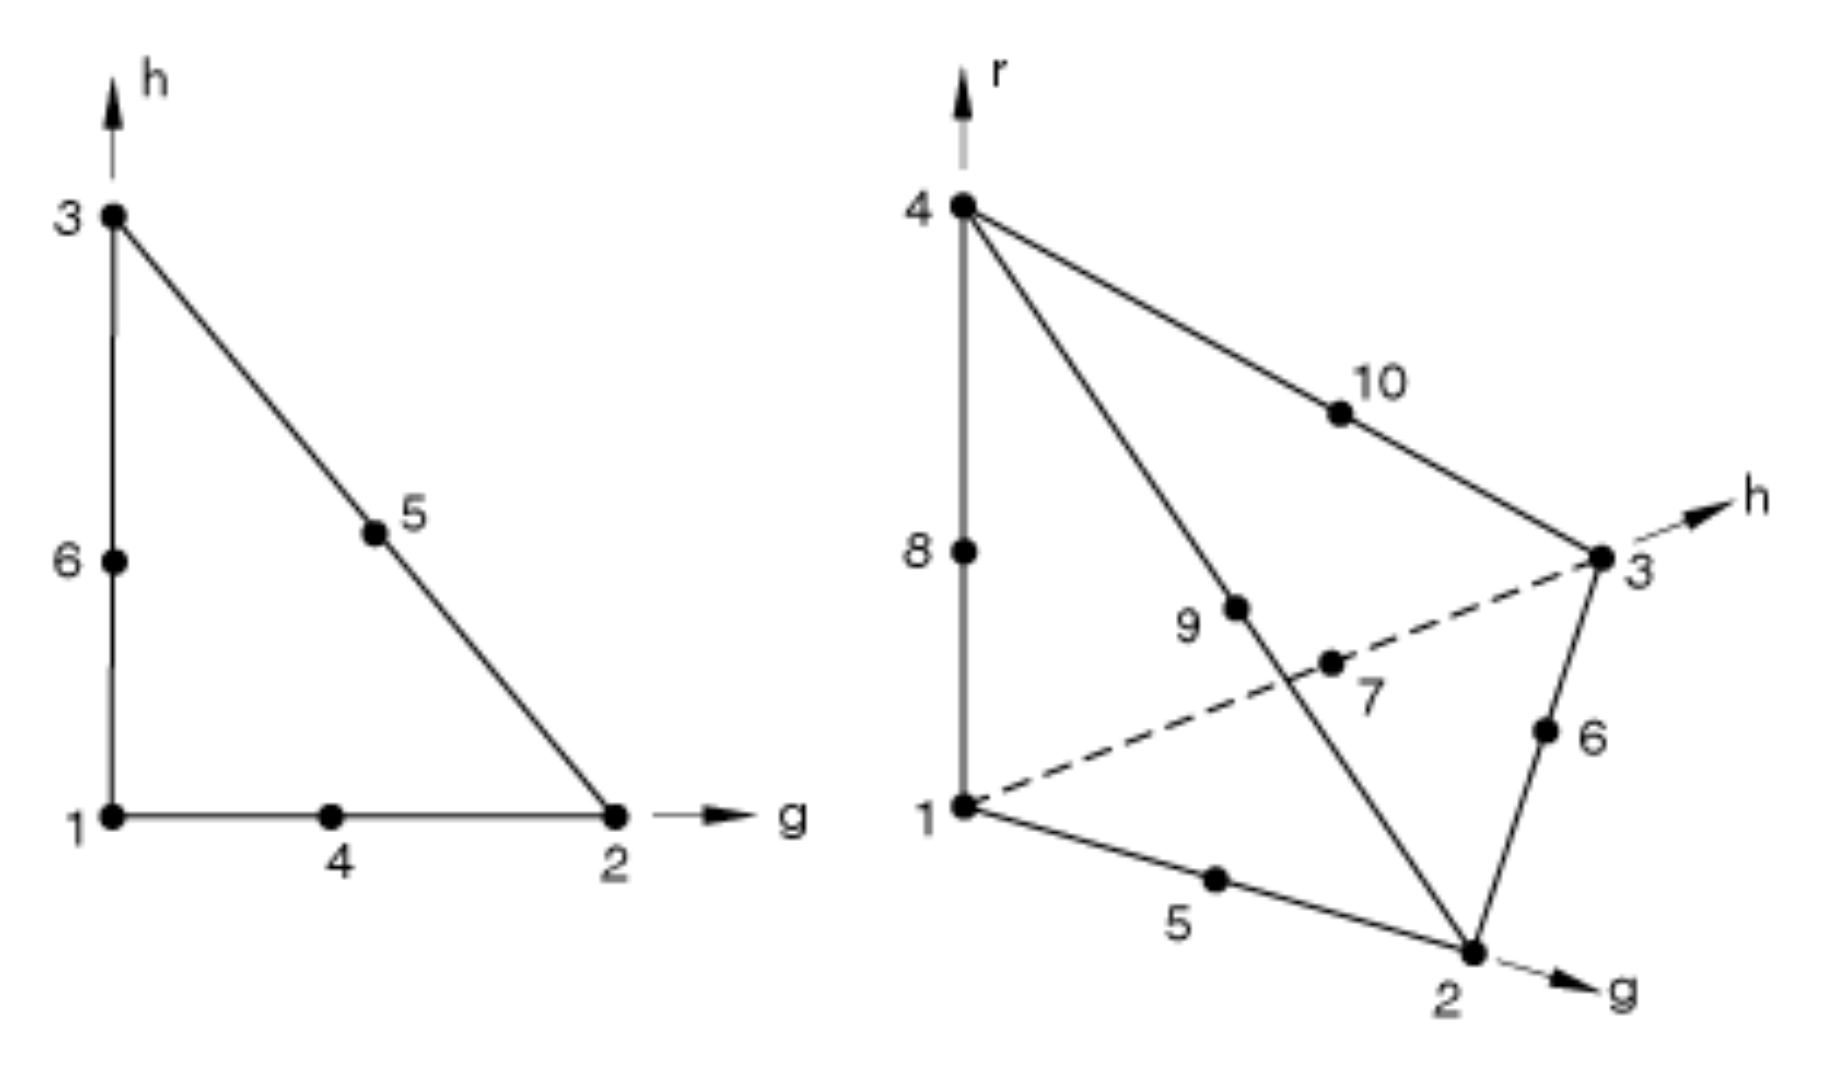
\includegraphics[width=11cm]{isoparametric_elements.png}
	\caption{Diagram showing the node numbering for the second order triangular and tetrahedral elements within Abaqus (CPS6 and C3D10 respectively).}
	\label{fig:isoparametric_elements}
\end{figure}

\subsection{Integration Point Coordinates}

It was necessary to determine the coordinates of each integration point in order to calculate their weights -- as the weight was based on the distance between the integration point and the inner radius of the domain. The shape functions calculated in the previous step defined the integration point coordinates in the natural coordinate system. These were then combined with the nodal coordinates for each element in order to define the integration point coordinates in the global coordinate system, using Equation \ref{eq:integration_point_coords}.

\begin{equation}\label{eq:integration_point_coords}
	\bm{p} = \bm{S} \cdot \bm{n}
\end{equation}

\begin{itemize}
	\item $\bm{p}$ is a matrix of shape $(n_{ip}, n_{dim})$ containing the integration point coordinates for the element.
	\item $\bm{S}$ is a matrix of shape $(n_{ip}, n_{nodes})$ containing the numerical evaluations of the shape functions in the natural coordinate system for the element.
	\item $\bm{n}$ is a matrix of shape $(n_{nodes}, n_{dim})$ containing the nodal coordinates for the element.
	\item $n_{nodes}$, $n_{ip}$, and $n_{dim}$ are the number of nodes per element, the number of integration points per element, and the dimensions of each element respectively. These are $(6, 3, 2)$ for CPS6 elements, and $(10, 3, 3)$ for C3D10 elements.
\end{itemize}

\subsection{Jacobian Matrices \& Determinants}

The Jacobian matrix gives the mapping between a set of coordinates in the natural (reference) coordinate system and the same relative coordinates within the global (deformed) coordinate system  -- it effectively maps the shape of the undeformed element to the shape of the deformed element. The Jacobian determinant is simply the determinant of the Jacobian matrix, and gives the ratio of the area or volume of the undeformed element to that of the deformed element. As the formulation for J-integral is an integration over $dA$ or $dV$ (for 2D and 3D elements respectively), the Jacobian determinant was therefore necessary in order to perform the integration -- as using the undeformed areas or volumes would introduce inaccuracies. The Jacobian matrix was calculated using a similar equation to Equation \ref{eq:integration_point_coords}, but using the shape function derivatives in place of the shape functions themselves. This equation is presented in Equation \ref{eq:jacobian_matrix}. The Jacobian determinant was then trivial to calculate, by taking the determinant of $\bm{J}$.

\begin{equation}\label{eq:jacobian_matrix}
	\bm{J} = \frac{\partial\bm{N}}{\partial\bm{\xi}} \cdot \bm{n}
\end{equation}

\begin{itemize}
	\item $\bm{J}$ is a 3D tensor of shape $(n_{ip}, n_{dim}, n_{dim})$ containing the Jacobian matrix for each integration point within the element.
	\item $\frac{\partial\bm{N}}{\partial\bm{\xi}}$ is a 3D tensor of shape $(n_{ip}, n_{nodes}, n_{dim})$ containing the numerical evaluations of the shape function derivatives in the natural coordinate system for the element.
	\item $\bm{n}$ is a matrix of shape $(n_{nodes}, n_{dim})$ containing the nodal coordinates for the element.
	\item $n_{nodes}$, $n_{ip}$, and $n_{dim}$ are the number of nodes per element, the number of integration points per element, and the dimensions of each element respectively. These are $(6, 3, 2)$ for CPS6 elements, and $(10, 3, 3)$ for C3D10 elements.
\end{itemize}


\subsection{Strain Energy Density}

The strain energy density was calculated for each integration point of each element, using the stress and strain tensors extracted from Abaqus for that integration point. This was accomplished using Equation \ref{eq:strain_energy_density}

\begin{equation}\label{eq:strain_energy_density}
	W = 0.5\ \bm{\sigma}_{ij}\ \bm{\epsilon}_{ij}
\end{equation}

\begin{itemize}
	\item $\bm{\sigma}_{ij}$ is the stress tensor
	\item $\bm{\epsilon}_{ij}$ is the strain tensor
\end{itemize}

\subsection{Displacement Gradients}

The displacement gradients represent the spatial derivatives of the displacement field, and effectively quantify how the displacement varies throughout an element. They are later combined with the stress tensor to determine the work done within the material as part of the J-integral expression. The first step in calculating the displacement gradients was to convert the shape function derivatives were to the global (deformed) coordinate system, using Equation \ref{eq:global_derivs}

\begin{equation}\label{eq:global_derivs}
	\frac{\partial \bm{N}}{\partial \bm{x}} = \left(\bm{J}^{-1} \left(\frac{\partial \bm{N}}{\partial \bm{\xi}}\right)^T \right)^T
\end{equation}

\begin{itemize}
	\item $\frac{\partial \bm{N}}{\partial \bm{x}}$ is a matrix of shape $(n_{dim}, n_{dim})$, containing the shape function derivatives in the global (deformed) coordinate system for each integration point.
	\item $\frac{\partial \bm{N}}{\partial \bm{\xi}}$ is a matrix of shape $(n_{nodes}, n_{dim})$ containing shape function derivatives in the natural (reference) coordinate system for each integration point.
	\item $\bm{J^{-1}}$ is a matrix of shape $(n_{dim}, n_{dim})$, and the inverse of the Jacobian matrix $\bm{J}$.
\end{itemize}

The displacement gradients at each integration point were then calculated by combining the shape function derivatives in the global (deformed) coordinate system with the nodal displacements for each element, using Equation \ref{eq:displacement_grads}.

\begin{equation}\label{eq:displacement_grads}
	\frac{\partial \bm{u}}{\partial \bm{x}} = \bm{U}^{T} \cdot \frac{\partial \bm{N}}{\partial \bm{x}}
\end{equation}

\begin{itemize}
	\item $\frac{\partial \bm{u}}{\partial \bm{x}}$ is a matrix of shape $(n_{dim}, n_{dim})$ representing the displacement gradient at the integration point.
	\item $\bm{U}$ is a matrix of shape $(n_{nodes}, n_{dim})$ containing nodal displacement values.
	\item $\frac{\partial \bm{N}}{\partial \bm{x}}$ is a matrix of shape $(n_{nodes}, n_{dim})$ containing global shape function derivatives.
\end{itemize}

\subsection{Weight Functions}\label{sec:weight_functions}

Weight functions are used within the domain integral method in order to apply different weights to each element or integration point within the domain, thereby increasing or decreasing the significance of their contribution relative to that of other elements or integration points. The actual weight function used can be arbitrary, providing that it is a smooth function that is equal to one at the inner radius of the domain, and is equal to zero at the outer radius of the domain. Three weight functions were used within the analysis in order to perform a comparison -- linear, polynomial, and Gaussian functions were used. The first step was to define the normalised distance of each integration point within the domain, using the parameters presented in Figure \ref{fig:domain_definition}.

\begin{figure}[H]
	\centering
	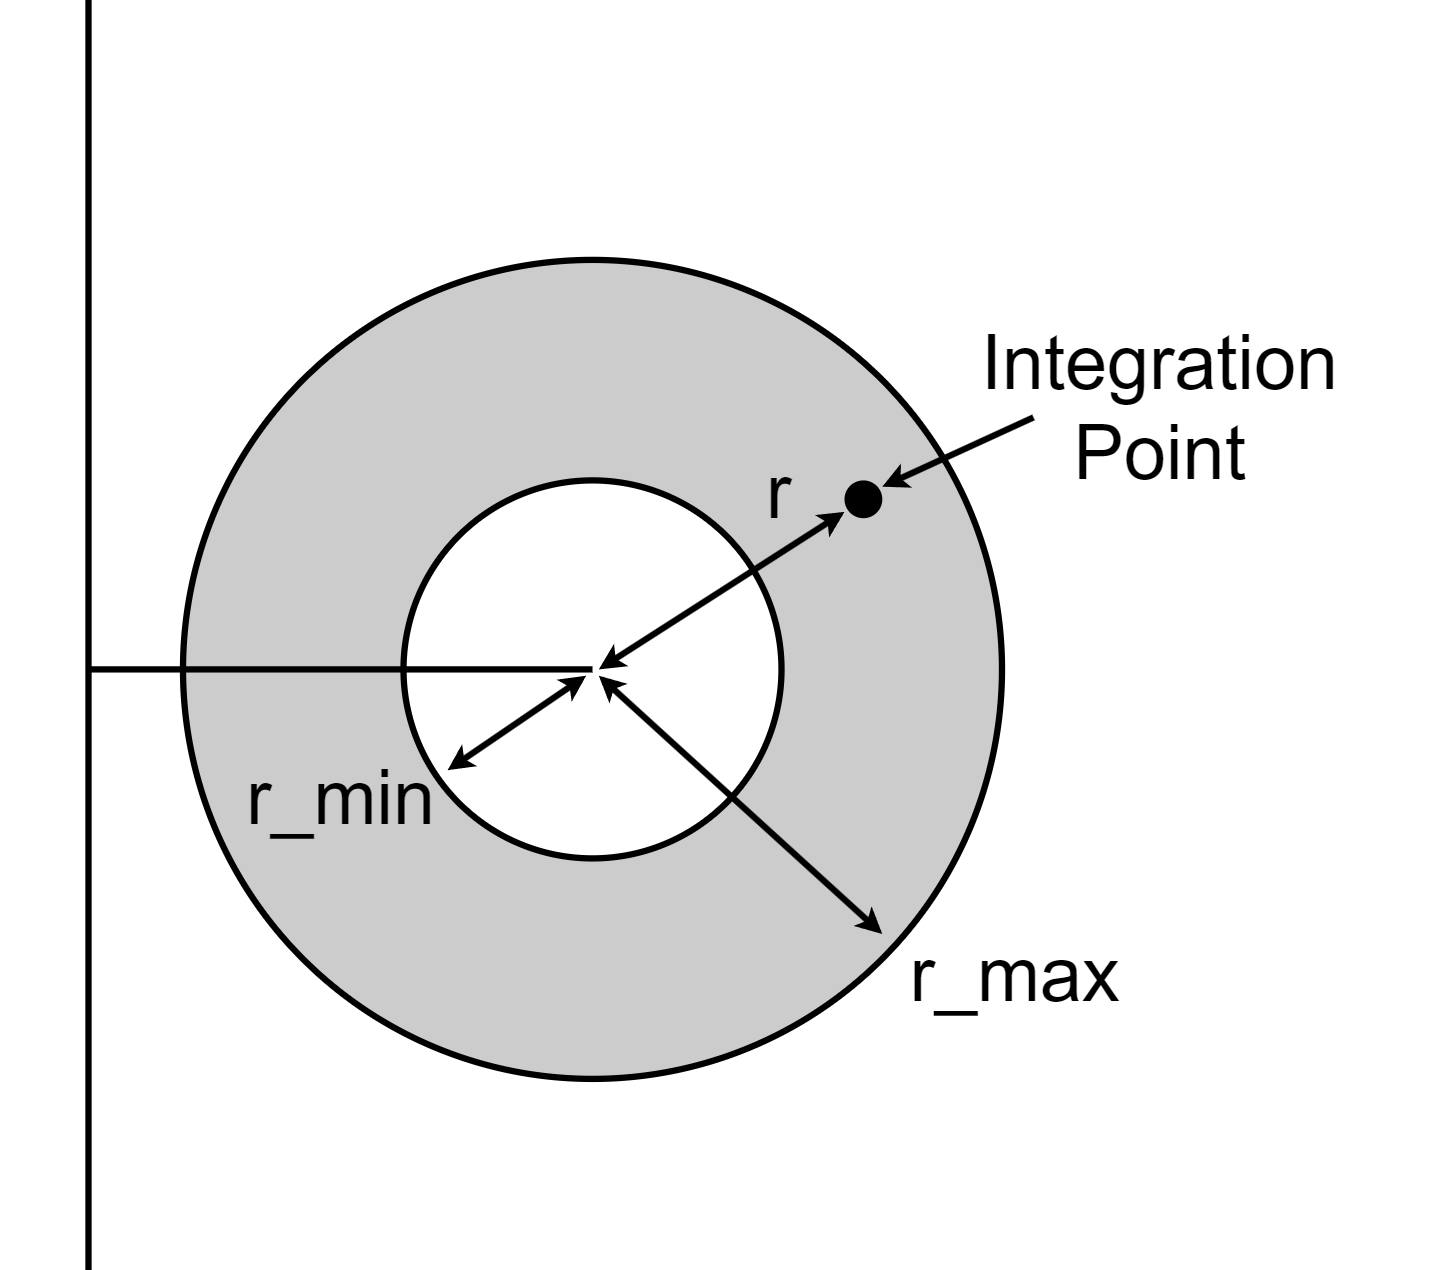
\includegraphics[width=11cm]{domain_definition.png}
	\caption{Diagram showing the measurements used to calculate the weight of each integration point using the weight function. The crack is the horizontal line perpendicular to the left edge of the part, while the grey-shaded annular region is the domain.}
	\label{fig:domain_definition}
\end{figure}

The normalised distance was effectively the relative position of the integration point within the domain -- for example, a normalised distance of 0.75 would signify that the integration point was 75\% of the way through the domain. This distance was defined as $s$, and was calculated using Equation \ref{eq:normalised_distance}.

\begin{equation}\label{eq:normalised_distance}
	s = \frac{r - r_{min}}{r_{max} - r_{min}}
\end{equation}

The normalised distance was then used to calculate the weight functions using the equations below. The derivatives of each function were also calculated by hand and defined as variables within the software. The linear weight function and its derivatives are given in Equations \ref{eq:weight_function_linear} and \ref{eq:weight_function_deriv_linear}.

\begin{equation}\label{eq:weight_function_linear}
	q = 1 - s
\end{equation}

\begin{equation}\label{eq:weight_function_deriv_linear}
	\frac{dq}{dr} = \frac{-1}{r_{max} - r_{min}}
\end{equation}

A polynomial of degree 3 was selected for the polynomial weight function. The polynomial weight function and its derivatives are given in Equations \ref{eq:weight_function_poly} and \ref{eq:weight_function_deriv_poly}.

\begin{equation}\label{eq:weight_function_poly}
	q = 1 - 3s^2 + 2s^3
\end{equation}

\begin{equation}\label{eq:weight_function_deriv_poly}
	\frac{dq}{dr} = \frac{-6s + 6s^2}{r_{max} - r_{min}}
\end{equation}

Finally, a Gaussian weight function was specified with a constant of 2.5, which was found to provide the best agreement with published results for the J-integral. The Gaussian weight function and its derivatives are given in Equations \ref{eq:weight_function_gauss} and \ref{eq:weight_function_deriv_gauss}.

\begin{equation}\label{eq:weight_function_gauss}
	q = \rm e^{-2.5s^2}
\end{equation}

\begin{equation}\label{eq:weight_function_deriv_gauss}
	\frac{dq}{dr} = \frac{-2.5s \cdot \rm e^{-2.5s^2}}{r_{max} - r_{min}}
\end{equation}

\subsection{J-Integral Calculation}

The previously calculated values were then combined in order to calculate the J-integral for each domain. The domain formulation of the J-integral was first presented in Equation \ref{eq:j_integral_2d}. However, this continuous equation could not be directly implemented using the finite element analysis results, so it was therefore necessary to convert it to a discrete form, which allowed summation over each element and integration point. The discrete form is given in Equation \ref{eq:j_integral_2d_eval}.

\begin{equation}\label{eq:j_integral_2d_eval}
	J = \sum_{e=1}^{e=n_{e}} \sum_{i=1}^{i=n_{ip}} \left[ \sigma_{ij}\frac{\partial u_i}{\partial x_1} - W\,\delta_{1j} \right]\frac{\partial q}{\partial x_j}\, \cdot \det J \cdot w_{ip}
\end{equation}

\begin{itemize}
	\item $n_e$ is the number of elements within the domain.
	\item $n_{ip}$ is the number of integration points within each element (excluding integration points which sat outside the domain).
	\item $\det J$ is the Jacobian determinant at the integration point.
	\item $w_{ip}$ is the integration point weight, obtained from the element formulation ($\frac{1}{6}$ for CPS6 elements and $\frac{1}{24}$ for C3D10 elements \cite{aster_111_nodate}).
\end{itemize}

During the evaluation of the integral, the actual area of the element was not necessary -- it's impact was accounted for by the Jacobian determinant and the integration point weights. The Jacobian determinant described the ratio between the original area of the element and the deformed area, and the integration point weight described the ratio between the area accounted for by the integration point, and the total area of the reference element. For example, a triangular CPS6 element has a reference area of $\frac{1}{2}$, given that a triangle occupies half of the area of a $1 \times 1$ unit square. Since the CPS6 element contains three integration points, the weight of each integration point is therefore $\frac{1}{2} \times \frac{1}{3} = \frac{1}{6}$.

\subsection{Stress Intensity Factor Calculation}

As the plate used for the analysis was 100 mm in height, 50 mm in width, and 1 mm in thickness, an assumption of plane stress could be made. Equally, as the plate was subjected to purely tensile loading, the assumption that only Mode I crack opening occurred could also be made. The equation for the stress intensity factor was presented in Equation \ref{eq:sif}. An analytical solution was obtained for the configuration factor $\beta_{i}$ for an edge crack in a finite-width plate with a uniform tensile load, and is presented in Equation \ref{eq:beta_edge_crack} \cite{yuan_research_2023}.

\begin{equation}\label{eq:beta_edge_crack}
	\beta_I = 1.12 - 0.23 \left(\frac{a}{b}\right) + 10.6 \left(\frac{a}{b}\right)^2 - 21.7 \left(\frac{a}{b}\right)^3 + 30.4 \left(\frac{a}{b}\right)^4
\end{equation}

\begin{itemize}
	\item $a$ is the crack length,
	\item $b$ is the plate width
\end{itemize}

This configuration factor could then be substituted into Equation \ref{eq:sif} in order to obtain the equations for $K_I$ specific to the analysed configuration, which was dependent on the crack length. A function was created to calculate the stress intensity factor via the analytical equation -- as well as via the J-integral obtained from the analysis -- so that the values could be compared. A percentage error was also calculated.






